\subsection{Ondas estacionárias de som no tubo de Rubens}

Nessa prática, iremos utilizar um Tubo de Rubens para a obtenção da velocidade do som em um gás. Colocaremos o GLP (gás liquefeito do petróleo – utilizado como gás de cozinha) em nosso tubo e vamos variar a frequência f, para a obtenção de diferentes harmônicos – começando pelo harmônico fundamental (n = 1). O comprimento L do tubo será mantido constante em todo o experimento. 

\[L = 1,45 +- 0,01 m\]

Podemos calcular o lambda  $\lambda$ para cada harmônico (n) do experimento, utilizando a seguinte reação:

\[ L = n \cdot \frac{\lambda _n}{2}\]

Portanto, teremos:

\[ 1,45 = 1 \cdot \frac{\lambda _1}{2} \ \to \ \lambda _1 = 2,90 m  \]
\[ 1,45 = 2 \cdot \frac{\lambda _2}{2} \ \to \ \lambda _2 = 1,45 m  \]
\[ 1,45 = 3 \cdot \frac{\lambda _3}{2} \ \to \ \lambda _3 = 0,967 m  \]
\[ 1,45 = 4 \cdot \frac{\lambda _4}{2} \ \to \ \lambda _4 = 0,725 m  \]
\[ 1,45 = 5 \cdot \frac{\lambda _5}{2} \ \to \ \lambda _5 = 0,580 m  \]

A incerteza de $\lambda _n$ será:

\[ L = n \cdot \frac{\delta \lambda _n}{2}\]

Assim, podemos calcular a incerteza para cada $\lambda _n$:

\[ 0,01 = 1 \cdot \frac{\delta \lambda _1}{2} \ \to \  \delta \lambda _1 = 0,02 m  \]
\[ 0,01 = 2 \cdot \frac{\delta \lambda _2}{2} \ \to \  \delta \lambda _2 = 0,01 m  \]
\[ 0,01 = 3 \cdot \frac{\delta \lambda _3}{2} \ \to \  \delta \lambda _3 = 0,007 m  \]
\[ 0,01 = 4 \cdot \frac{\delta \lambda _4}{2} \ \to \  \delta \lambda _4 = 0,005 m  \]
\[ 0,01 = 5 \cdot \frac{\delta \lambda _5}{2} \ \to \  \delta \lambda _5 = 0,004 m  \]

Com todos os comprimentos de onda $\lambda _n$ e suas incertezas calculados, podemos tomar as frequências $f_n$ -- formadoras dos diferentes harmônicos -- apresentadas nos vídeos e montar uma tabela com todas essas informações  :\\


\begin{table}[H]
    \centering
    \begin{tabular}{ |M{3cm}||M{3cm}||M{4.2cm}||M{3.5cm}|  }
        \hline
        \textbf{Índice (\textit{n}) do harmônico } & \textbf{Número de nós} & \textbf{Lambda {$\lambda _n$} (m)}  & \textbf{Frequência {$f_n$} (Hz)}\\
        \hline 
         1&	1&	2,90  $\pm$  0,02 	& 94,81 \\
         
         2&	2&	1,45  $\pm$  0,01   & 193,22\\
         
         3&	3&	0,967 $\pm$  0,007  &	293,61\\
         
         4&	4&	0,725  $\pm$ 0,005  &	387,27\\
         
         5&	5&	0,580  $\pm$ 0,004  &	474,26\\
        \hline
    \end{tabular}
    \caption{Tabela registrando os valores do índice do harmônico, o número de nós, $\lambda _n$ e \textit{$f_n$}}
\end{table}

Agora, podemos construir um gráfico de $f_n$ versus n/2L. Para isso, utilizaremos outra tabela para nos organizarmos, baseada na tabela acima, mas agora relacionando a frequência com n/2L:


\begin{table}[H]
    \centering
    \begin{tabular}{ |M{5cm}||M{5cm}||M{4cm}|  }
        \hline
        \textbf{Índice (\textit{n}) do harmônico } & \textbf{Frequência {$f_n$} (Hz)} & \textbf{n/2L}\\
        \hline 
         1 & 94,81 	& 0,34483\\
         2 & 193,22 & 0,68966\\
         3 & 293,61	& 1,03448\\
         4 & 387,27 & 1,37931\\
         5 & 474,26	&1,72414\\
        \hline
    \end{tabular}
    \caption{Tabela que relaciona a frequência \textit{$f_n$} com n/2L}
\end{table}

Agora, somos capazes de montar o gráfico sem maiores complicações:

\begin{figure}[H]
  \centering
  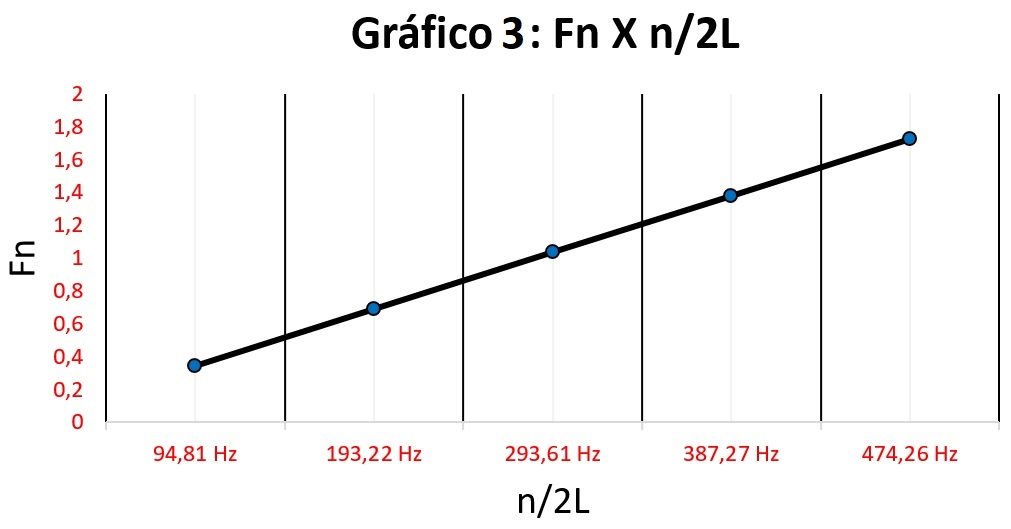
\includegraphics[scale=0.7]{images/Graf2.jpg}
  \caption{Gráfico de $f_n$ versus n/2L}
\end{figure}
